\documentclass[aspectratio=169]{beamer}

\usetheme{Madrid}
\usecolortheme{seahorse}
\usepackage[utf8]{inputenc}
\usepackage{listings}
\usepackage{xcolor}
\usepackage{graphicx}
\usepackage{booktabs}

\lstdefinestyle{cli}{
  basicstyle=\ttfamily\scriptsize,
  backgroundcolor=\color{black!5},
  frame=single,
  breaklines=true,
  columns=fullflexible,
  keywordstyle=\color{blue},
}
\lstnewenvironment{cli}{\lstset{style=cli}}{}

\title{EDA Tool Options, Explained for Dummies}
\subtitle{Every real CLI flag and environment variable openPDKcreator passes to each real tool -- what it does, in plain language, and why}
\author{}
\date{}

\begin{document}

\frame{\titlepage}

% ---------------------------------------------------------------
\begin{frame}{What this deck is}
\begin{itemize}
  \item openPDKcreator's own Library Manager has ``Open in X'' buttons
        for Magic, xschem, KLayout, and Qucs-S -- plus a real,
        indirect path to ngspice, Netgen, Yosys, OpenROAD, and
        LibreLane. Each real launch is a real command line: a binary,
        some flags, maybe an environment variable.
  \item This deck explains \emph{every single one of those}, tool by
        tool, assuming zero prior knowledge of any of them -- what
        the flag is called, what it actually does, and why this
        project passes exactly that one and not something else.
  \item For each of the four real, interactive GUIs (Magic, xschem,
        KLayout, Qucs-S) it also goes one level further: a real
        ``menu bar, tab by tab'' table covering \emph{every single
        real top-level menu} that tool's own GUI actually has, opened
        live and read directly -- not just the launch flags, but what
        you'd actually see once the window is open.
  \item Nothing here is guessed. Every claim was checked directly
        against each real tool's own \texttt{--help}/\texttt{-h}
        output, its own real, installed man page, its own real menu
        bar (opened live, screenshotted, read), or (where none of
        those existed) its own real, fetched source code -- and
        several real, live screenshots below are real bugs this
        project found and fixed \emph{because} of that checking.
  \item If you've never used a terminal-based EDA tool before, start
        with the next slide. If you already know what a CLI flag and
        an environment variable are, skip straight to Magic.
\end{itemize}
\end{frame}

% ---------------------------------------------------------------
\begin{frame}[fragile]{Building blocks, for total beginners}
\begin{itemize}
  \item \textbf{A CLI flag} is a word starting with \texttt{-} or
        \texttt{--} that changes how a program behaves, e.g.\
        \texttt{-e} below turns on editing:
\begin{cli}
klayout -e mychip.gds
\end{cli}
  \item \textbf{A positional argument} is anything on the command
        line \emph{without} a leading dash -- usually a file name.
        Above, \texttt{mychip.gds} is one: ``open this file''.
  \item \textbf{An environment variable} is a named value the
        \emph{whole shell session} carries, which any program started
        from it can read -- set with \texttt{export NAME=value}, read
        inside a program as \texttt{\$NAME} (shell) or via that
        program's own real API (e.g.\ Python's \texttt{os.environ}).
        Unlike a flag, it's invisible on the command line itself.
  \item \textbf{Batch mode} means ``run without a GUI, do the job, and
        exit'' -- no window ever opens; the opposite of
        \textbf{interactive mode}, where a real window stays open for
        a human to click around in.
  \item \textbf{A startup/init file} (often called an ``rc file'',
        short for ``run commands'') is a real script a program reads
        automatically every time it starts, before doing anything
        else -- convenient for a human's own personal preferences,
        dangerous when a program assumes \emph{whose} preferences
        those are. Most of this deck is about exactly that risk.
\end{itemize}
\end{frame}

% =================================================================
\section{Magic}
\begin{frame}{Magic -- what it is}
\begin{itemize}
  \item A real, 1980s-vintage-but-still-actively-developed
        \textbf{layout editor}: draws real polygons on real GDS
        layers, and can \textbf{extract} a real netlist (which shapes
        touch which, turned into transistors/devices/nets) from a
        real drawn layout.
  \item Everything Magic draws or extracts is only meaningful
        relative to one specific \textbf{technology} -- the real set
        of layers, electrical rules, and device-recognition rules for
        one specific real fab process (or, here, one from-scratch
        demo process). Get the technology wrong and Magic still
        opens, still lets you draw -- it just silently means
        something else's rules the whole time.
\end{itemize}
\end{frame}

% ---------------------------------------------------------------
\begin{frame}[fragile]{Magic -- the real flags this project passes}
\begin{cli}
magic -d XR -rcfile <path-to-.magicrc> <script-or-file>
\end{cli}
\begin{itemize}
  \item \texttt{-d XR} -- which real graphics driver to use.
        \texttt{XR} means ``X11, real color'' -- the normal choice on
        Linux; irrelevant to correctness, just how pixels get drawn.
  \item \texttt{-rcfile <file>} -- \emph{use this exact real Tcl
        script as the startup file}, instead of Magic's own default
        search (its compiled-in system directory, then the current
        directory). This is the one real flag this whole deck is
        about: whichever file you name here is what tells Magic which
        real technology to load.
  \item The trailing \texttt{<script-or-file>} is either a real,
        freshly-generated Tcl script (see next slide) or, for
        IHP's own real PDK, its own official
        \texttt{ihp-sg13g2.magicrc} (documented verbatim in that
        PDK's own \texttt{libs.tech/magic/README.md}, not derived).
\end{itemize}
\textbf{A flag this project deliberately does \emph{not} use:}
\texttt{-T <technology>} looks up a technology \emph{by name} in
Magic's own fixed search locations (current directory, then
\texttt{\$CAD\_ROOT}) -- it cannot be pointed at an arbitrary real
path the way \texttt{-rcfile}'s own \texttt{tech load} command can, so
it can't address a real project living anywhere on disk.
\end{frame}

% ---------------------------------------------------------------
\begin{frame}[fragile]{Magic -- the real bug this project found}
Before this project's own real fix, opening a cell for a \emph{new},
from-scratch project (no \texttt{.magicrc} of its own yet) generated a
script with no technology line at all -- Magic then silently fell back
to auto-sourcing whatever \texttt{.magicrc} its own compiled
default/environment happened to find. In this project's own real dev
container, that turned out to be \textbf{IHP's own sg13g2}
technology, not the actual project being worked on:
\begin{cli}
gds read <path>
load <cell>
\end{cli}
The real, working fix: always prepend one real line, found via this
project's own \texttt{extraction.default\_tech\_file()} (the
shortest-stem real \texttt{.tech} file under \texttt{libs.tech/magic/}):
\begin{cli}
tech load <real, absolute path to the correct .tech file>
gds read <path>
load <cell>
\end{cli}
\end{frame}

% ---------------------------------------------------------------
\begin{frame}{Magic -- the real bug, live}
\begin{columns}
\column{0.5\textwidth}
\centering
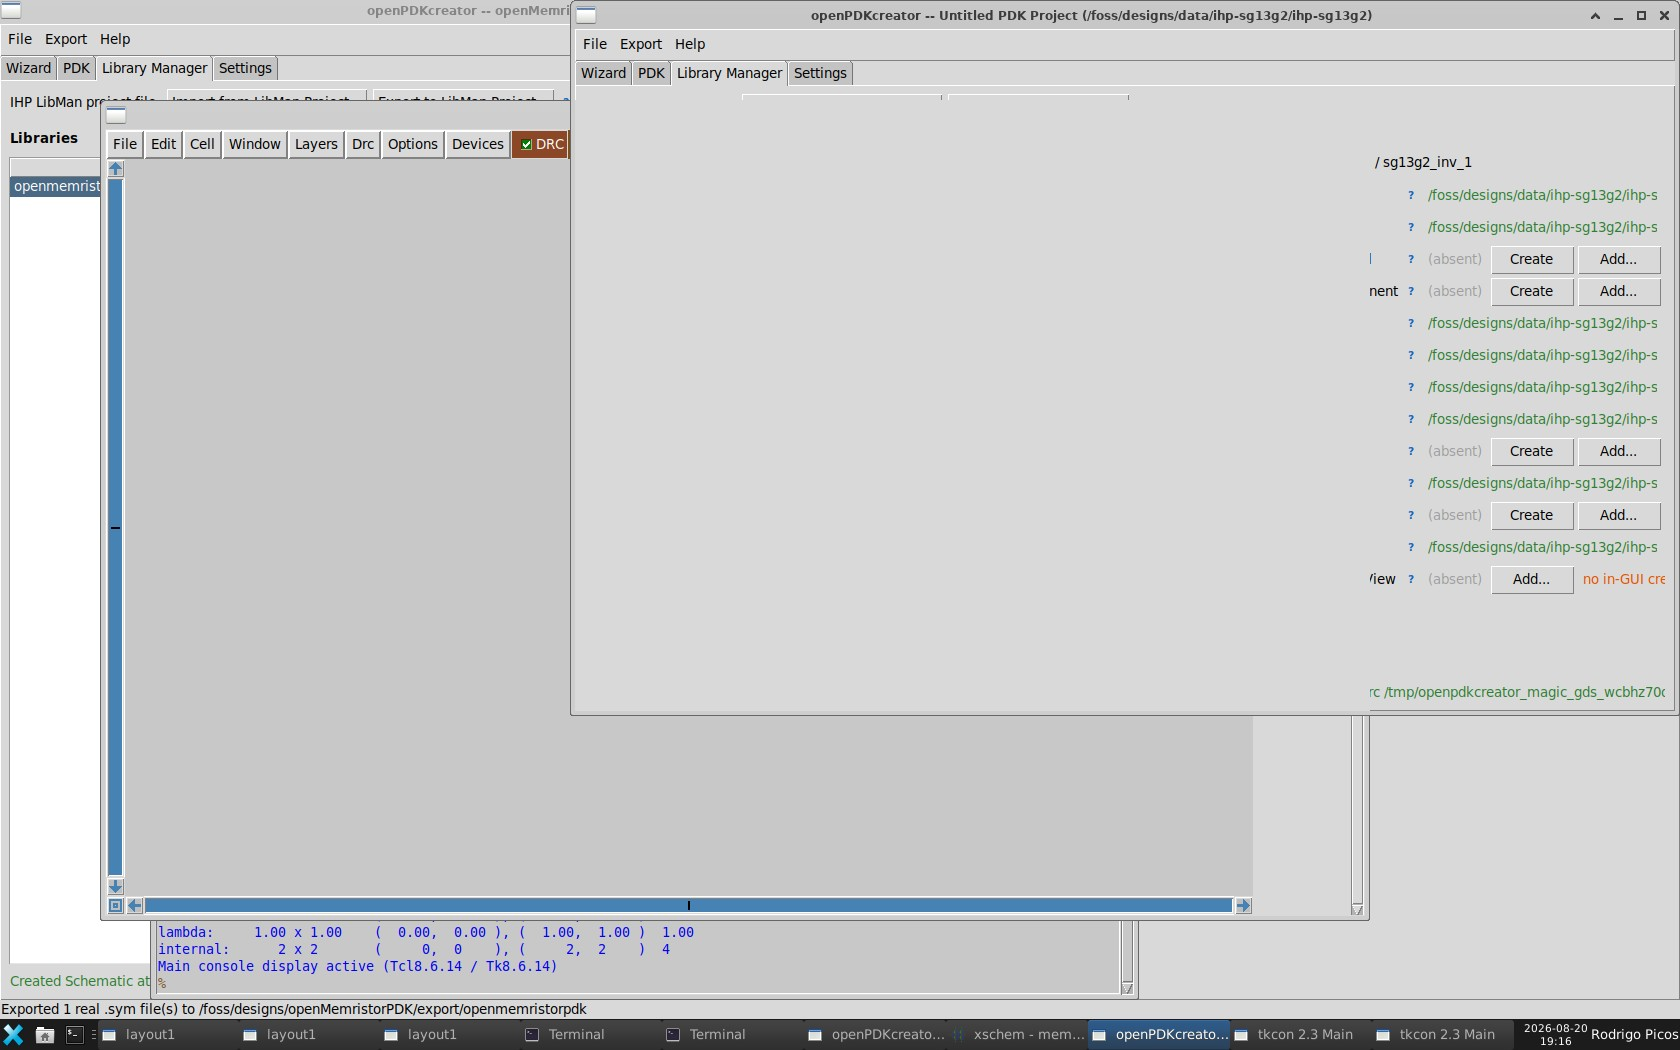
\includegraphics[width=\textwidth]{figures/tooldeck_magic_wrong_tech.jpg}
\footnotesize Before the fix: title bar reads
\texttt{Technology: ihp-sg13g2} -- wrong real technology, real layer
panel shows IHP's own layers, for a memristor project.
\column{0.5\textwidth}
\centering
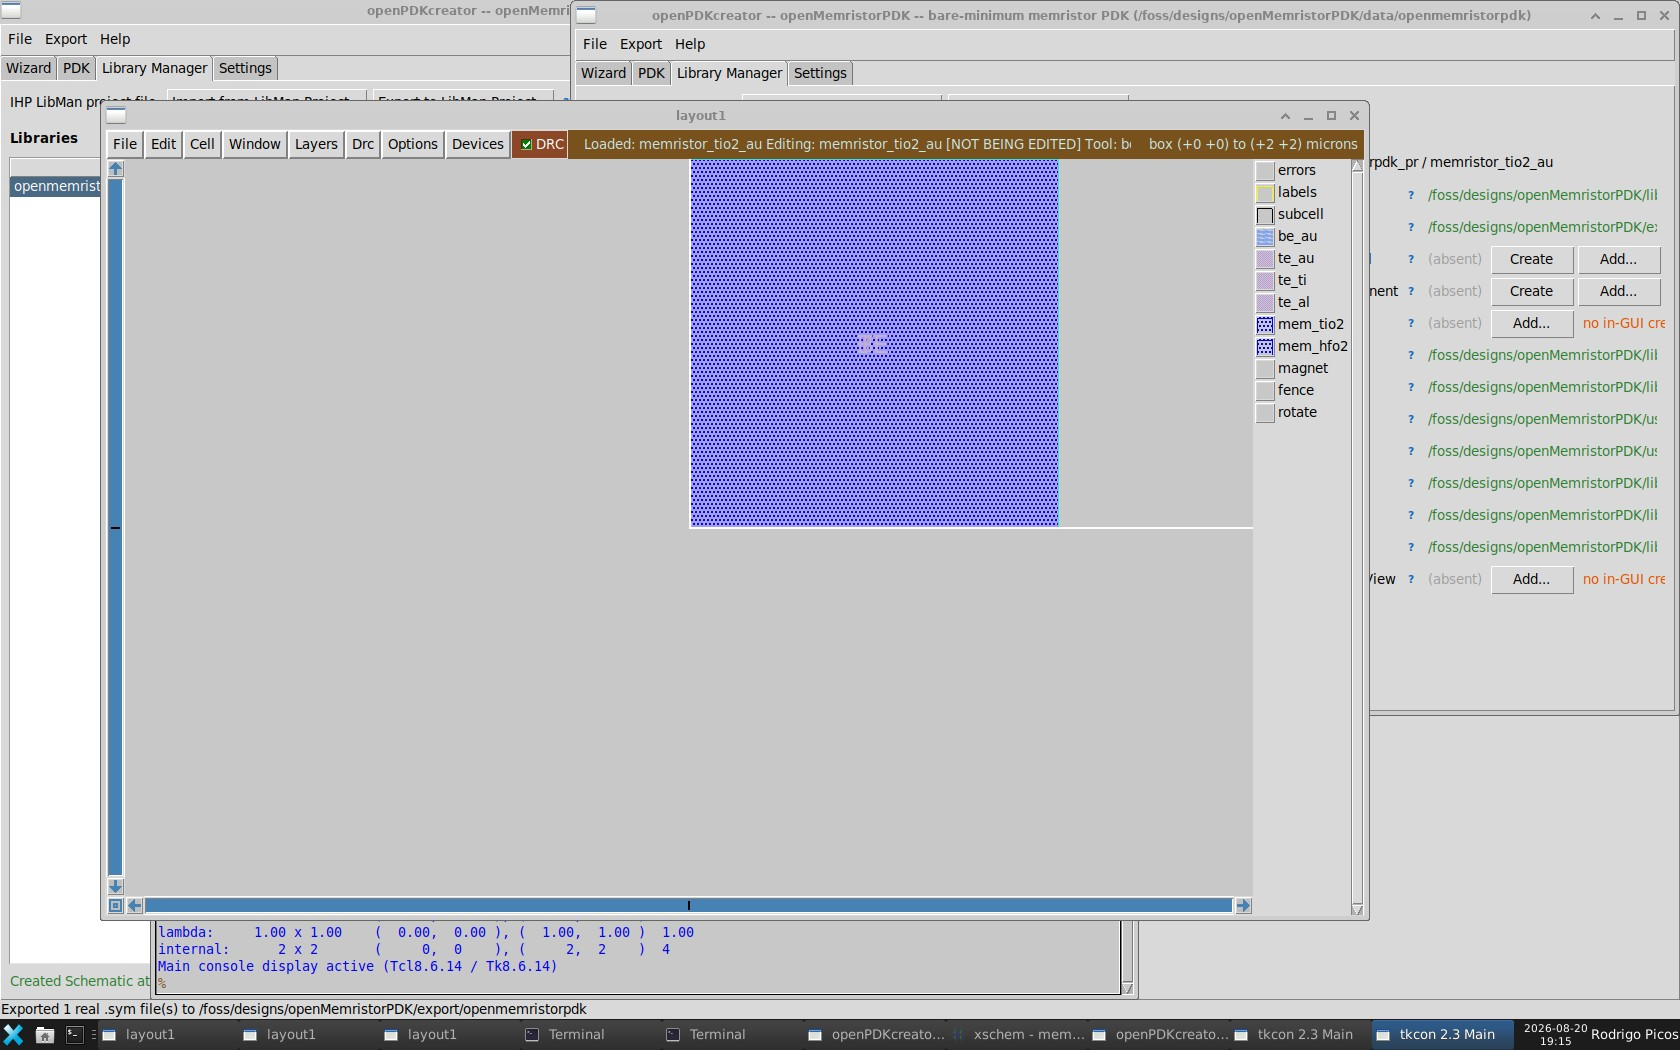
\includegraphics[width=\textwidth]{figures/tooldeck_magic_correct_tech.jpg}
\footnotesize After: title bar reads
\texttt{Technology: openmemristorpdk}, real layer panel shows
\texttt{be\_au}/\texttt{te\_au}/\texttt{mem\_tio2}/\dots -- this
project's own real layers, correctly loaded.
\end{columns}
\end{frame}

% ---------------------------------------------------------------
\begin{frame}[fragile]{Magic's own menu bar, tab by tab}
Every one of Magic's own real top-level menus, opened live and read
directly (not from memory) -- what each is actually for:
\footnotesize
\begin{center}
\begin{tabular}{ll}
\toprule
Real menu & What it's actually for \\
\midrule
File & Open/Save a real \texttt{.mag}; Import SPICE; Read/Write GDS \\
Edit & Undo/Redo, Delete, real rotate/mirror/move/stretch \\
Cell & New/Save cell; hierarchy navigation; Expand/Lock a real cell \\
Window & New/clone view; real zoom/grid controls, per-window \\
Layers & Protect/Unlock base layers; Reorder layers \\
Drc & Run/report DRC, interactively (this project's own real
      \textbf{Run DRC} button instead runs it in real batch mode) \\
Options & Toggle real sub-panels -- Cell/Library/Tech/DRC Manager,
          Netlist Window, 3D Display \\
Devices & A real, parameterized device generator (MOSFETs, diodes,
           resistors, \dots) -- IHP-supplied content here, not
           generic Magic, and not this project's own real memristor
           device (which has none of these) \\
\bottomrule
\end{tabular}
\end{center}
\normalsize
\end{frame}

% =================================================================
\section{xschem}
\begin{frame}{xschem -- what it is}
\begin{itemize}
  \item A real \textbf{schematic capture} tool: draws symbols (a
        device's outline plus its real pins) and schematics (symbols
        wired together with real nets), and can turn a real schematic
        into a real SPICE netlist for simulation.
  \item Like Magic, xschem needs to know where a project's own real
        symbol library lives -- otherwise its own real ``place a
        component'' browser has nothing of this project's own to
        show, and any menu customizations another real PDK ships
        (see the case study below) leak in instead.
\end{itemize}
\end{frame}

% ---------------------------------------------------------------
\begin{frame}[fragile]{xschem -- the real flags this project passes}
\begin{cli}
xschem --rcfile <path-to-real-rc-file> <symbol-or-schematic-file>
\end{cli}
\begin{itemize}
  \item \texttt{--rcfile <file>} -- real, documented (its own man
        page, since \texttt{--help} prints nothing useful in this
        container): ``Use \texttt{<file>} as a rc file for startup
        instead of the default xschemrc.'' Replaces xschem's own
        default startup chain outright, rather than adding to it.
  \item The trailing file is a plain positional argument -- the
        symbol/schematic to open. xschem has \emph{no} separate flag
        for ``open this specific file''; it's always just the last
        thing on the command line.
  \item Two flags this project does \emph{not} pass, on purpose:
        \texttt{-i}/\texttt{--no\_rcload} (skip \emph{every} rc file,
        including this project's own real one -- too blunt) and
        \texttt{--tcl <script>} (run arbitrary Tcl before startup --
        more power than this one, narrow job needs).
\end{itemize}
Inside that real rc file, the one line that actually matters:
\begin{cli}
append XSCHEM_LIBRARY_PATH :<this project's own real libs.tech/xschem>
\end{cli}
\end{frame}

% ---------------------------------------------------------------
\begin{frame}[fragile]{xschem -- the real bug this project found}
This dev container's own real, global
\texttt{\textasciitilde/.xschem/xschemrc} (part of the base image, not
this project) unconditionally sources
\texttt{\$PDK\_ROOT/\$PDK/libs.tech/xschem/xschemrc}, with
\texttt{PDK\_ROOT}/\texttt{PDK} hardcoded container-wide to IHP's own
real values. A plain \texttt{xschem <file>} launch, for \emph{any}
project, silently inherited IHP's own real symbol library path --
\emph{and} its own real custom ``IHP'' menu (a real, useful set of
IHP-specific shortcuts that PDK ships in
\texttt{libs.tech/xschem/xschem-menu}, sourced by its own real
\texttt{xschemrc}). The real, working fix: a project-specific
\texttt{--rcfile} that appends the right real library path, and
sources \emph{this} project's own \texttt{xschem-menu} \emph{if it
ships one} -- found generically, by real, on-disk presence, never by
hardcoding ``IHP'' anywhere in this project's own code. IHP's own real
project gets its own real menu back; a project that ships none, like
this one, gets nothing extra.
\end{frame}

% ---------------------------------------------------------------
\begin{frame}{xschem -- the real bug, live}
\begin{columns}
\column{0.5\textwidth}
\centering
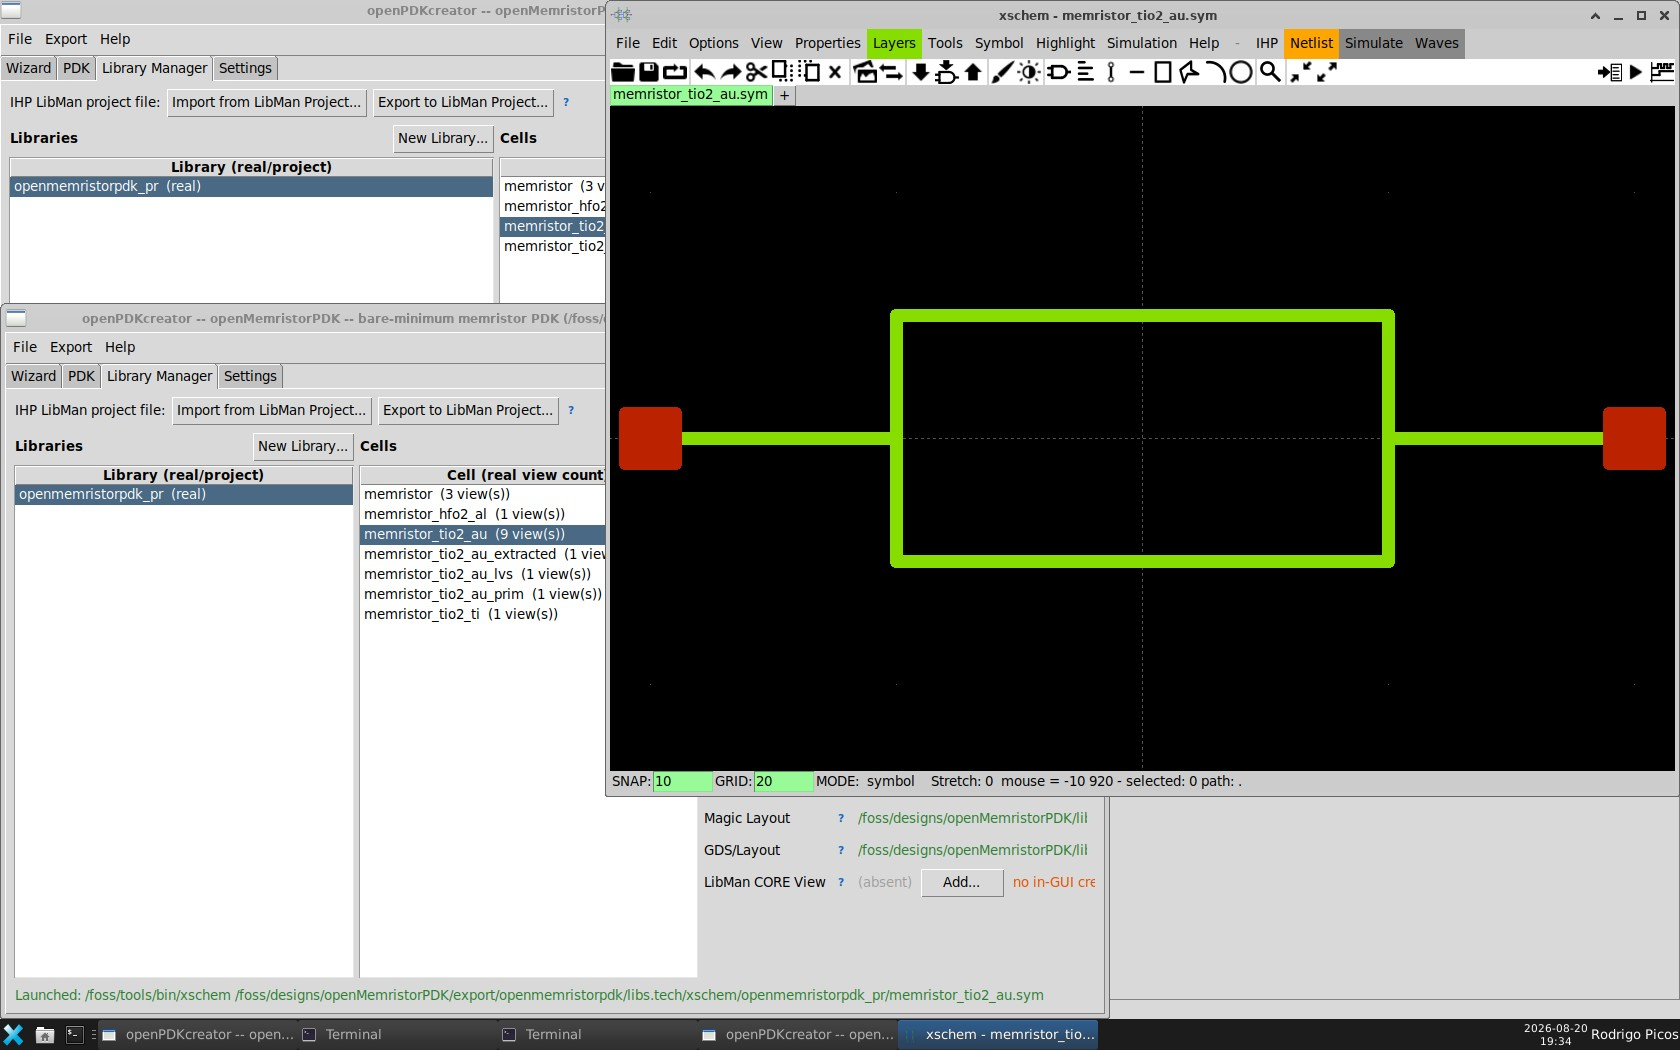
\includegraphics[width=\textwidth]{figures/tooldeck_xschem_ihp_menu.jpg}
\footnotesize Before the fix: a real, spurious \textbf{IHP} menu
between Help and Netlist -- for a memristor project's own symbol.
\column{0.5\textwidth}
\centering
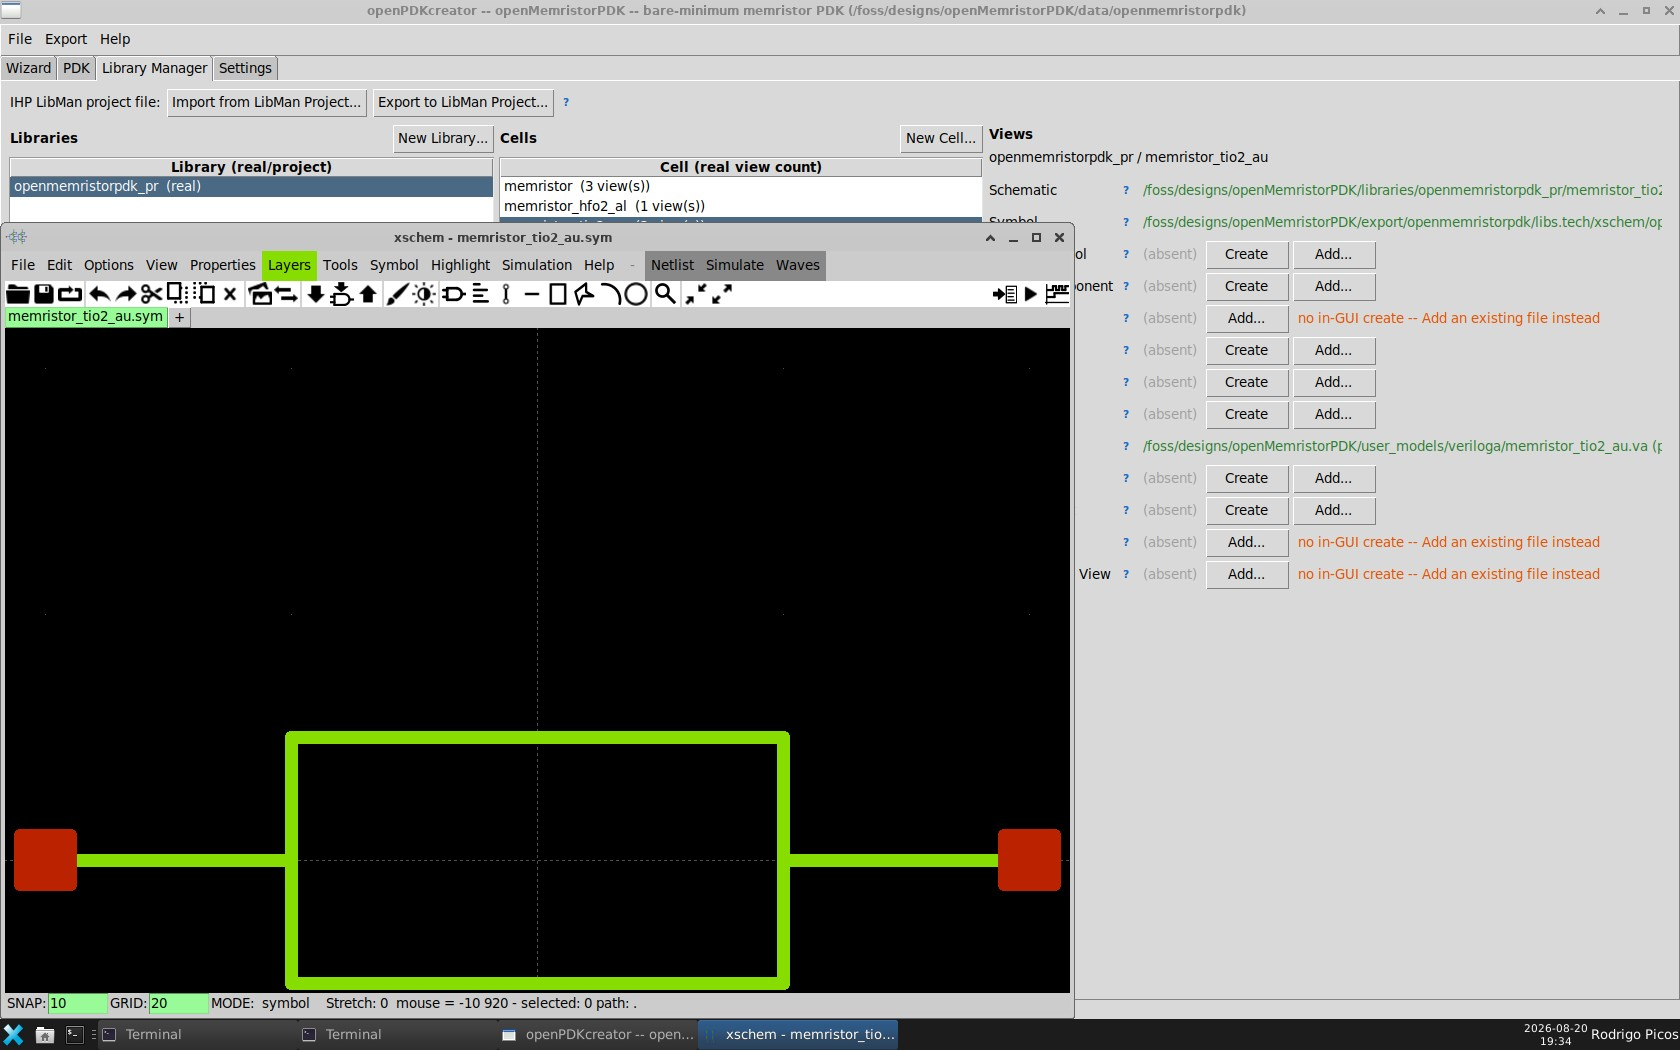
\includegraphics[width=\textwidth]{figures/tooldeck_xschem_correct.jpg}
\footnotesize After: no IHP menu, the exact same real symbol, status
bar showing the real \texttt{--rcfile <path>} that fixed it.
\end{columns}
\end{frame}

% ---------------------------------------------------------------
\begin{frame}[fragile]{xschem's own menu bar, tab by tab (1/2)}
\footnotesize
\begin{center}
\begin{tabular}{ll}
\toprule
Real menu & What it's actually for \\
\midrule
File & Open/Save/Reload a real schematic or symbol; Component
       browser; Image export \\
Edit & Undo/Redo, Copy/Cut/Paste; real move/rotate/flip; Push/Pop
       into a real subcircuit hierarchy \\
Options & Real drawing/wiring preferences -- e.g.\ orthogonal
           wiring, auto-join wires, GPU workarounds; not this
           deck's own real \texttt{XSCHEM\_LIBRARY\_PATH} fix, which
           lives in the rc file instead, not here \\
View & Real zoom/redraw; toggle real side panels (Layers, Cells,
       Libraries); line width/colorscheme \\
Properties & Edit a real selected object's own real attributes --
              including the real, deliberately red
              \textbf{Edit file (danger!)} entry, a genuine, honest
              in-GUI warning \\
\bottomrule
\end{tabular}
\end{center}
\normalsize
\end{frame}

% ---------------------------------------------------------------
\begin{frame}[fragile]{xschem's own menu bar, tab by tab (2/2)}
\footnotesize
\begin{center}
\begin{tabular}{ll}
\toprule
Real menu & What it's actually for \\
\midrule
Layers & A real, numbered (0--19) drawing-layer color palette --
          which real layer new lines/text land on next \\
Symbol & Make symbol$\leftrightarrow$schematic; place real pins/
         ports/net labels \\
Highlight & Real net/pin highlighting; compare two real schematics
            side by side \\
Simulation & \textbf{Configure simulators and tools} -- the real
              in-GUI counterpart to this deck's own
              \texttt{ngspice}/\texttt{osdi} discussion; also
              real netlist-directory and LVS settings \\
Help & Real keybinding reference; About \\
\bottomrule
\end{tabular}
\end{center}
\normalsize
Three real, one-click \textbf{action buttons} sit to the right of the
menu bar, not inside it -- \textbf{Netlist}/\textbf{Simulate}/
\textbf{Waves} each just runs, immediately, rather than opening a
dropdown (confirmed live: clicking \textbf{Netlist} here really did
generate a real \texttt{.spice} file on the spot).
\end{frame}

% =================================================================
\section{KLayout}
\begin{frame}{KLayout -- what it is}
\begin{itemize}
  \item A real, modern \textbf{layout viewer/editor} and
        \textbf{DRC engine} (Design Rule Checking -- confirming a
        real layout obeys a real process's own real geometric limits,
        via a real, scriptable Ruby/Python API).
  \item Used two real, different ways in this project: interactively
        (\textbf{Open in KLayout}, a human looking at a real cell) and
        in real batch mode (\textbf{Run DRC}, no human, just a
        pass/fail report).
\end{itemize}
\end{frame}

% ---------------------------------------------------------------
\begin{frame}[fragile]{KLayout -- interactive flags this project passes}
\begin{cli}
klayout -l <path-to-.lyp> -rr <path-to-generated-pya-script>
\end{cli}
\begin{itemize}
  \item \texttt{-l <file>} -- real, stable flag: load this real
        ``layer properties'' file (names/colors/display styles for
        every real layer) for anything opened afterward.
  \item \texttt{-rr <script>} -- run this real Python
        (\texttt{pya}) script at startup, \emph{but don't exit
        afterward} (plain \texttt{-r} would run it then quit;
        \texttt{-rm} would run it \emph{before} any file is loaded,
        too early for this project's own real ``jump to this cell''
        script to have anything loaded yet to act on).
  \item Deliberately \emph{not} passed: \texttt{-e} (editable mode) --
        \textbf{Open in KLayout} is real, plain \emph{viewer} mode by
        this project's own design; real editing happens in Magic/
        xschem instead.
  \item \texttt{-n <technology>}/\texttt{-nn <file>} (pick/point at a
        technology) exist too, but this project's own real script
        already gets the right layer names via \texttt{-l} alone, so
        neither is needed here.
\end{itemize}
\end{frame}

% ---------------------------------------------------------------
\begin{frame}[fragile]{KLayout -- batch-mode flags (Run DRC)}
\begin{cli}
klayout -b <path-to-.gds> -r <path-to-.drc-script> -rd output=<report>
\end{cli}
\begin{itemize}
  \item \texttt{-b} -- \textbf{batch mode}: real, documented shorthand
        for \texttt{-zz -nc -rx} together (\texttt{-zz} = fully
        headless, database only, no window at all; \texttt{-nc} =
        don't read \emph{any} configuration file; \texttt{-rx} =
        ignore implicit macros). This is why \textbf{Run DRC} was
        never at risk of the same class of bug as Magic/xschem/
        Qucs-S: batch mode structurally can't read a hidden,
        container-wide default in the first place.
  \item \texttt{-r <script>} -- run this real DRC Ruby script (same
        real flag as the interactive case, just without
        \texttt{-rr}'s ``stay open'' behavior -- batch mode exits when
        the script finishes regardless).
  \item \texttt{-rd output=<path>} -- define a real Ruby/Tcl script
        variable (\texttt{\$output} inside the DRC script) -- this
        project's own real DRC deck reads it to know where to write
        the real report database.
\end{itemize}
\end{frame}

% ---------------------------------------------------------------
\begin{frame}[fragile]{KLayout -- the real \texttt{KLAYOUT\_HOME} lever}
KLayout's own real, documented environment variable
(\texttt{klayout -h} prints it):
\begin{cli}
KLAYOUT_HOME   The path to KLayout's data (configuration, macros,
               libraries etc). Default: ~/.klayout on Linux.
\end{cli}
This project's own \textbf{Open in KLayout} reuses one real,
persistent KLayout window across repeated clicks (the same real idea
IHP's own LibMan tool uses) via a small real Python script polling a
real ``command file''. The first real launch used to be blocked by two
real, first-use ``Tip'' dialogs (modal windows Python can't click
past) -- worked around, at first, with a synthetic keypress. Revisited
later: a fresh, real, per-project \texttt{KLAYOUT\_HOME} directory,
pre-seeded with the one real key that actually suppresses both real
dialogs (found by watching KLayout itself write it out, not guessed):
\begin{cli}
<tip-window-hidden>hide-empty-layers=4,hide-empty-layers=0,
                    editor-mode=4,editor-mode=0</tip-window-hidden>
\end{cli}
No dialog ever appears now -- the whole synthetic-keypress workaround
was deleted outright, a real simplification, not just a fix.
\end{frame}

% ---------------------------------------------------------------
\begin{frame}{KLayout -- the real Tip dialog, live}
\begin{center}
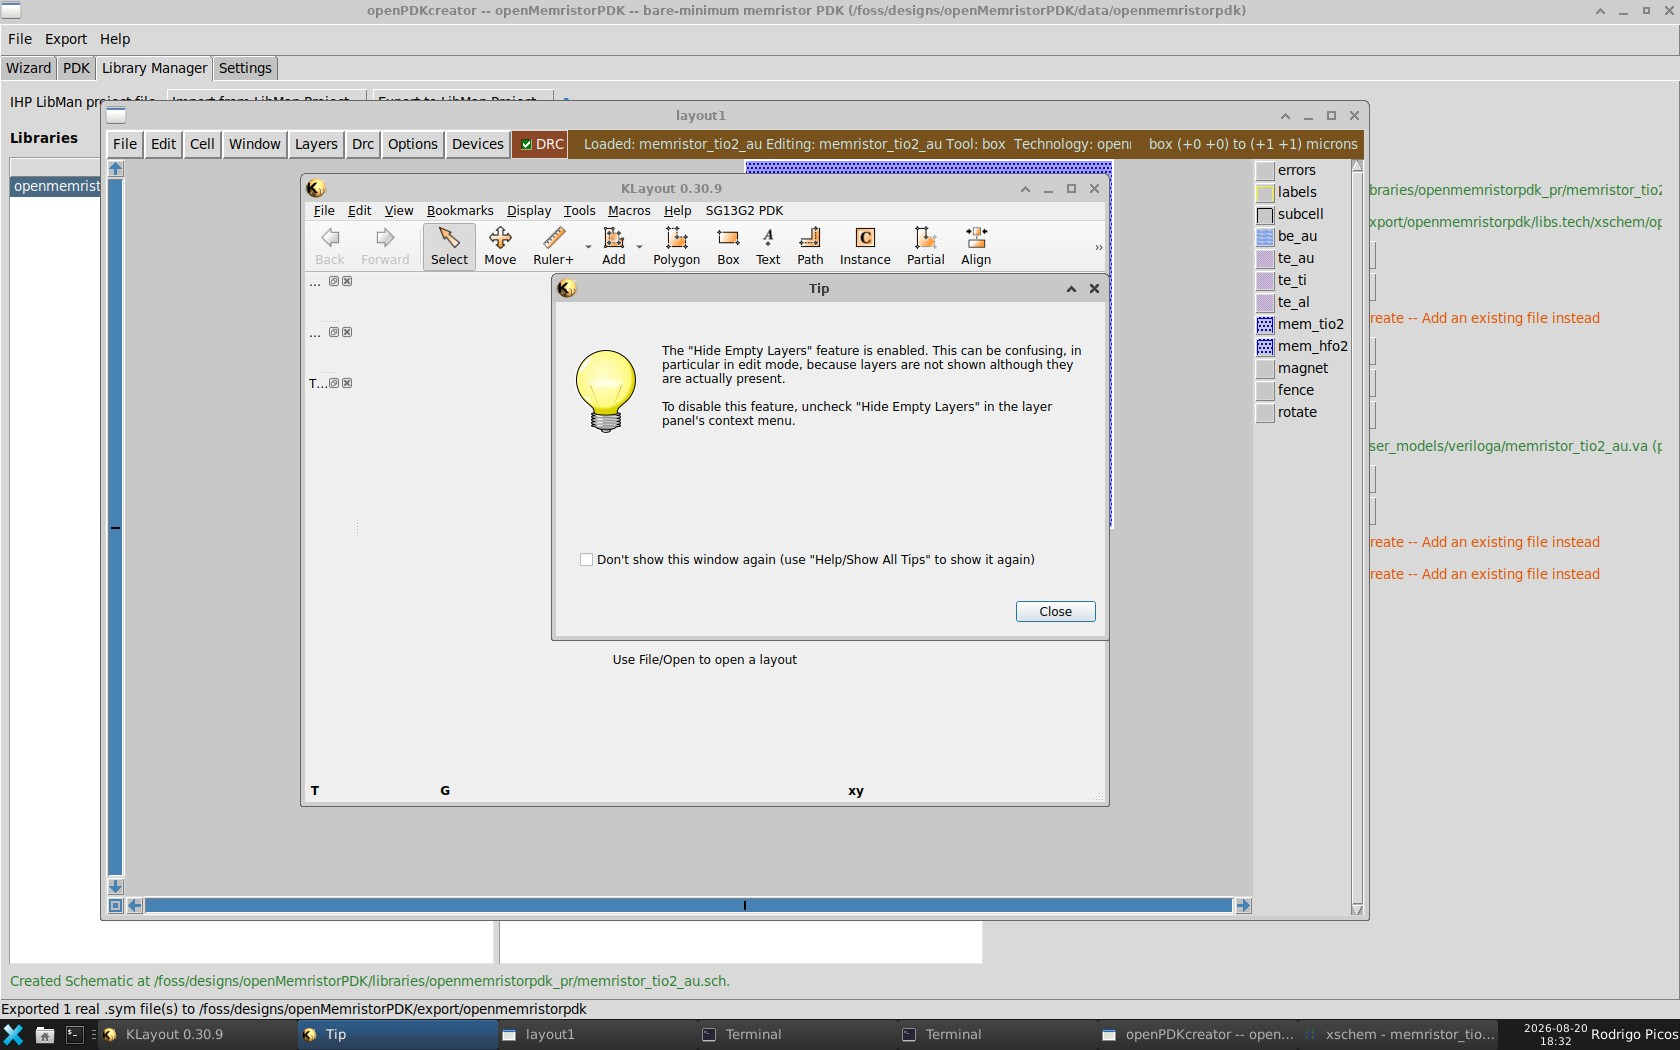
\includegraphics[width=0.62\textwidth]{figures/tooldeck_klayout_tip_dialog.jpg}
\end{center}
\footnotesize
The real, first-use ``Hide Empty Layers'' Tip dialog -- a real, modal
window that blocked this project's own real automation script from
ever running until dismissed, before \texttt{KLAYOUT\_HOME} pre-seeding
made it never appear at all.
\end{frame}

% ---------------------------------------------------------------
\begin{frame}[fragile]{KLayout's own menu bar, tab by tab}
\footnotesize
\begin{center}
\begin{tabular}{ll}
\toprule
Real menu & What it's actually for \\
\midrule
File & Open/Save a real layout; Screenshot; Load/Save real Layer
       Properties (the real GUI counterpart of this deck's own
       \texttt{-l <lyp>} flag) \\
Edit & Undo/Redo; real Layout/Cell/Layer/Selection editing;
       Search and Replace \\
View & Toggle real panels (Layers, Cells, Libraries, Navigator);
       grid/marker/text display \\
Bookmarks & Save/return to a real, named view position \\
Display & Real zoom/hierarchy depth (Full/Box Only/Top Level);
           Descend/Ascend into a real cell \\
Tools & \textbf{Manage Technologies} (the real GUI counterpart of
         \texttt{-n}/\texttt{-nn}/\texttt{KLAYOUT\_HOME}); real
         LVS/DRC/XOR/Diff tools; Netlist Browser \\
Macros & Real Ruby/Python macro editor -- the same real engine this
          project's own generated \texttt{pya} automation script
          (\textbf{Open in KLayout}'s persistent-instance mechanism)
          runs inside of \\
Help & \textbf{Show All Tips} -- the real, in-GUI way to re-enable
        the Tip dialogs this deck's own real
        \texttt{tip-window-hidden} fix suppresses \\
\bottomrule
\end{tabular}
\end{center}
\normalsize
\end{frame}

% =================================================================
\section{Qucs-S}
\begin{frame}{Qucs-S -- what it is}
\begin{itemize}
  \item A real, alternative \textbf{schematic capture + simulation}
        GUI (its own symbol/component format, distinct from xschem's).
  \item A real, confirmed, disclosed limit (checked directly against
        its own real, fetched \texttt{qucs/main.cpp}): there is
        \emph{no} real CLI way to open a specific file in its own
        interactive GUI. \texttt{-i FILENAME} is real, but only
        consulted in real batch \texttt{--netlist}/\texttt{--print}
        conversion mode -- with neither given, its own \texttt{main()}
        goes straight to \texttt{QucsMain->show()} and never even
        looks at \texttt{-i}. \textbf{Open in Qucs-S} says this
        plainly before launching, rather than glossing over it.
\end{itemize}
\end{frame}

% ---------------------------------------------------------------
\begin{frame}[fragile]{Qucs-S -- the real environment variable this project sets}
Since there's no file-opening flag to fix, the real, remaining
question is \emph{which workspace} Qucs-S opens into -- its own real
``Projects'' panel root, \texttt{QucsHomeDir}. That setting lives in
one real, shared, global config file
(\texttt{QSettings("qucs", "qucs\_s")} -- its own real, fetched
\texttt{settings.cpp} passes no explicit path, so Qt's own standard,
real \texttt{\$XDG\_CONFIG\_HOME}-aware lookup applies):
\begin{cli}
export XDG_CONFIG_HOME=<a real, disposable, per-launch temp directory>
qucs-s
\end{cli}
That temp directory holds a real \emph{copy} of the real, shared
config -- every other real setting (simulator paths, fonts) preserved
-- with only \texttt{QucsHomeDir=} swapped to this project's own real
\texttt{libs.tech/qucs-s}. The real, shared, original file is never
touched, so a different project's next real Qucs-S launch is
unaffected.
\end{frame}

% ---------------------------------------------------------------
\begin{frame}{Qucs-S -- the real fix, live}
\begin{center}
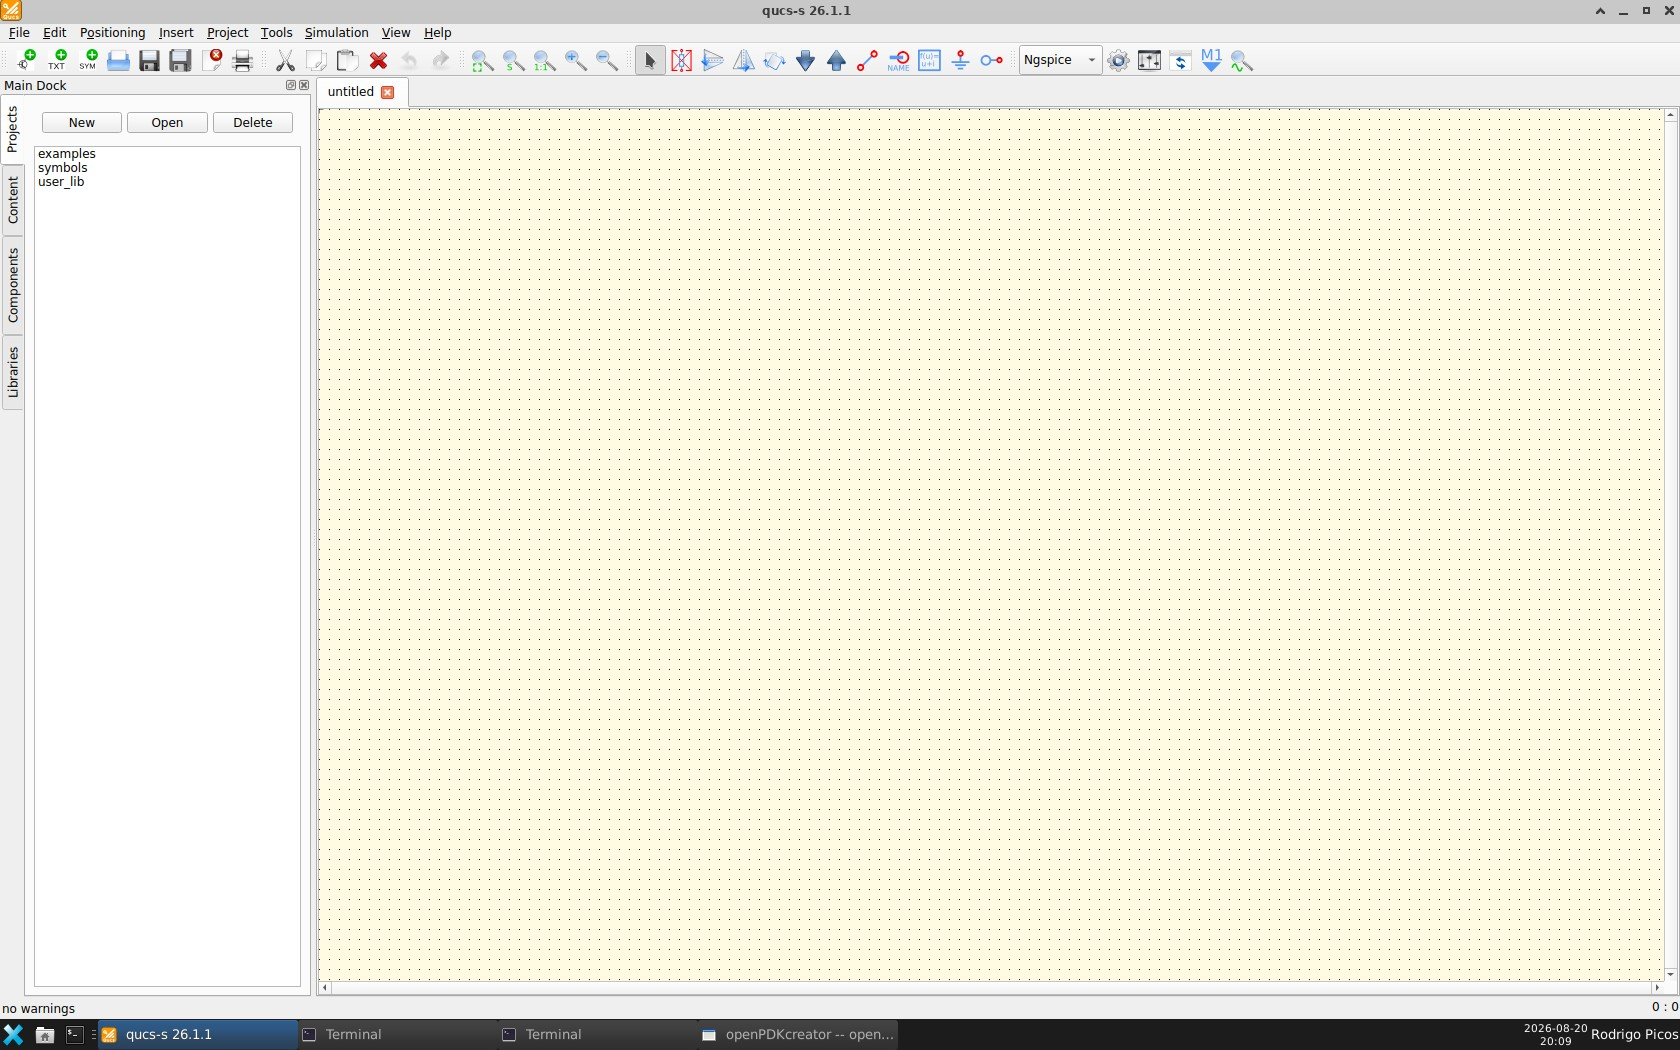
\includegraphics[width=0.55\textwidth]{figures/tooldeck_qucs_correct_workspace.jpg}
\end{center}
\footnotesize
The real Projects panel after the fix, correctly listing
\texttt{examples}/\texttt{symbols}/\texttt{user\_lib} -- this
project's own real \texttt{libs.tech/qucs-s} subdirectories, not the
dev container's own default \texttt{/headless/QucsWorkspace} (itself a
real symlink into IHP's own PDK install).
\end{frame}

% ---------------------------------------------------------------
\begin{frame}[fragile]{Qucs-S's own menu bar, tab by tab}
\footnotesize
\begin{center}
\begin{tabular}{ll}
\toprule
Real menu & What it's actually for \\
\midrule
File & Real Open/Save; \textbf{Application Settings} -- the real
       GUI's own version of this deck's own \texttt{QucsHomeDir} fix
       (edits the same real, shared config this project's own
       \texttt{\_qucs\_env()} copies instead of touching directly) \\
Edit & Real Cut/Copy/Paste; Move/Rotate/Mirror; Go into/Pop out of a
       real subcircuit \\
Positioning & Real align/center/distribute -- purely cosmetic,
               layout-only \\
Insert & Real Wire, Ground, Port, Equation, Marker placement \\
Project & \textbf{New/Open Project} -- browses from real
           \texttt{QucsHomeDir}, exactly the setting this deck's own
           real fix redirects; also real Verilog-A module build/load \\
Tools & A real RF-design toolbox -- filter/matching/attenuator
         synthesis, line calculation, S-parameters -- unrelated to
         this deck's own real launch-environment focus \\
Simulation & \textbf{Simulators Settings} -- the real GUI's own
              version of \texttt{qucs\_s.conf}'s
              \texttt{NgspiceExecutable}/\texttt{XyceExecutable}
              entries \\
View & Real zoom/grid/dock-window display \\
Help & Real Help Index, Getting Started, About \\
\bottomrule
\end{tabular}
\end{center}
\normalsize
\end{frame}

% =================================================================
\section{ngspice}
\begin{frame}[fragile]{ngspice -- what it is, and its real flags}
A real, industry-standard \textbf{SPICE circuit simulator} -- given a
real netlist (instances, values, sources, a \texttt{.tran}/\texttt{.dc}/
\texttt{.ac} analysis command), it solves the real circuit equations
and reports real voltages/currents over time or frequency.
\begin{cli}
ngspice -b mem_tran.sp
\end{cli}
\begin{itemize}
  \item \texttt{-b} -- real batch mode: run the given real netlist
        file and exit, no interactive prompt.
  \item ngspice auto-loads a real \texttt{.spiceinit} file from the
        \emph{current directory} at startup -- no CLI flag points at
        an arbitrary one, so this project always runs it from the
        real directory that file actually lives in.
  \item A real, confirmed OSDI (compiled Verilog-A model) requirement:
        \texttt{osdi <file>.osdi} must be loaded, inside a leading
        \texttt{.control}/\texttt{.endc} block, \emph{before} any
        \texttt{.model} card referencing it is parsed -- the real,
        documented fix for a real, otherwise-silent resolution
        failure is \texttt{pre\_osdi <file>.osdi} instead, which loads
        early enough even when a \texttt{.subckt} appears in the deck.
\end{itemize}
\end{frame}

% =================================================================
\section{Netgen}
\begin{frame}[fragile]{Netgen -- what it is, and its real flags}
A real \textbf{LVS} (Layout Versus Schematic) tool: compares two real
netlists -- one from a real, drawn layout (via Magic's own real
extraction), one from a real schematic/CDL reference -- and reports
whether they describe the same real circuit.
\begin{cli}
netgen -batch source <real, generated LVS setup script>
\end{cli}
\begin{itemize}
  \item \texttt{-batch} -- real, non-interactive mode: run the given
        real Tcl commands and exit, reporting a real pass/fail plus a
        real report file, never opening a window.
  \item \texttt{source <script>} -- Netgen's own real Tcl
        \texttt{lvs} command, naming both real netlists and their own
        real top-cell names, lives inside that generated script --
        this project writes it fresh, per real run, rather than
        maintaining one static file.
\end{itemize}
A real \textbf{pass} means more than matching pin lists: Netgen
confirms real \emph{device-level} equivalence -- the same real
component types, in the same real topology, not just the same real
names.
\end{frame}

% =================================================================
\section{Yosys}
\begin{frame}[fragile]{Yosys -- what it is, and its real flags}
A real \textbf{logic synthesis} tool: turns real Verilog RTL into a
real gate-level netlist, mapped onto a real standard-cell library.
\begin{cli}
yosys -c <script.tcl> -Q
\end{cli}
\begin{itemize}
  \item \texttt{-c <script>}/\texttt{-s <script>} -- run a real
        TCL/Yosys-native script of commands (\texttt{read\_verilog},
        \texttt{synth}, \texttt{write\_verilog}, \dots) instead of an
        interactive prompt.
  \item \texttt{-Q}/\texttt{-q}/\texttt{-qq} -- successively quieter
        logging (suppress the banner; only warnings/errors; only
        errors).
  \item \textbf{Confirmed genuinely safe by design}: Yosys's own real
        \texttt{--help} documents every real flag and environment
        variable it has, and \emph{none} of them refer to a default
        config file at all -- unlike every tool above, there is
        nothing here that could silently default to the wrong real
        PDK, because Yosys never reads anything it wasn't explicitly
        told to.
\end{itemize}
Not launched directly by this project's own Python code -- see
LibreLane, two slides on.
\end{frame}

% =================================================================
\section{OpenROAD}
\begin{frame}[fragile]{OpenROAD -- what it is, and its real flags}
A real \textbf{place-and-route} (PnR) and \textbf{static timing
analysis} (STA) tool: takes a real gate-level netlist and turns it
into a real, physical chip layout -- floorplanning, placement,
routing, timing closure.
\begin{cli}
openroad -exit -no_splash -metrics <path> <real tcl script>
\end{cli}
\begin{itemize}
  \item \texttt{-exit} -- exit after running the given real script
        (the interactive default is to stay open).
  \item \texttt{-no\_splash} -- skip the real license splash text.
  \item \texttt{-metrics <file>} -- write real, structured JSON
        metrics (timing, area, \dots) to this real path.
  \item \texttt{-no\_init} -- \textbf{skip a real
        \textasciitilde/.openroad Tcl file OpenROAD otherwise sources
        by default at startup} -- real, documented, but \emph{not}
        passed by LibreLane's own real, installed code (checked
        directly, not assumed), the tool that actually invokes
        OpenROAD in this project's own real flow. See next slide.
\end{itemize}
\end{frame}

% =================================================================
\section{LibreLane}
\begin{frame}[fragile]{LibreLane -- what it is, and its real flags}
A real \textbf{silicon-compiler orchestrator}: runs the whole real
RTL-to-GDS flow -- Yosys (synthesis), OpenROAD (PnR, STA), Magic/
KLayout (DRC), Netgen (LVS) -- as one real, reproducible pipeline of
steps, each one a real subprocess call to the tool that actually does
the work.
\begin{cli}
librelane --manual-pdk --pdk-root "$PDK_ROOT" --pdk "$PDK"
\end{cli}
\begin{itemize}
  \item \texttt{--manual-pdk} -- use a real, already-present PDK
        directory directly, skipping LibreLane's own default
        Ciel/Volare PDK-fetch mechanism entirely.
  \item \texttt{--pdk-root}/\texttt{--pdk} -- \emph{explicit, required}
        real arguments naming exactly which real PDK, and where.
        Structurally the safest tool in this whole deck: there is no
        silent fallback to get wrong in the first place, since
        LibreLane simply won't run without these.
\end{itemize}
This project's own real \texttt{librelane\_pdk()} shell wrapper
derives both values from whichever real project is currently loaded
(never hardcoded), and additionally runs in a real, fresh, isolated
\texttt{\$HOME} -- a defensive real fix, since LibreLane's own
internal OpenROAD calls never pass \texttt{-no\_init} (previous
slide).
\end{frame}

% ---------------------------------------------------------------
\begin{frame}{LibreLane -- the real fix, live}
\begin{center}
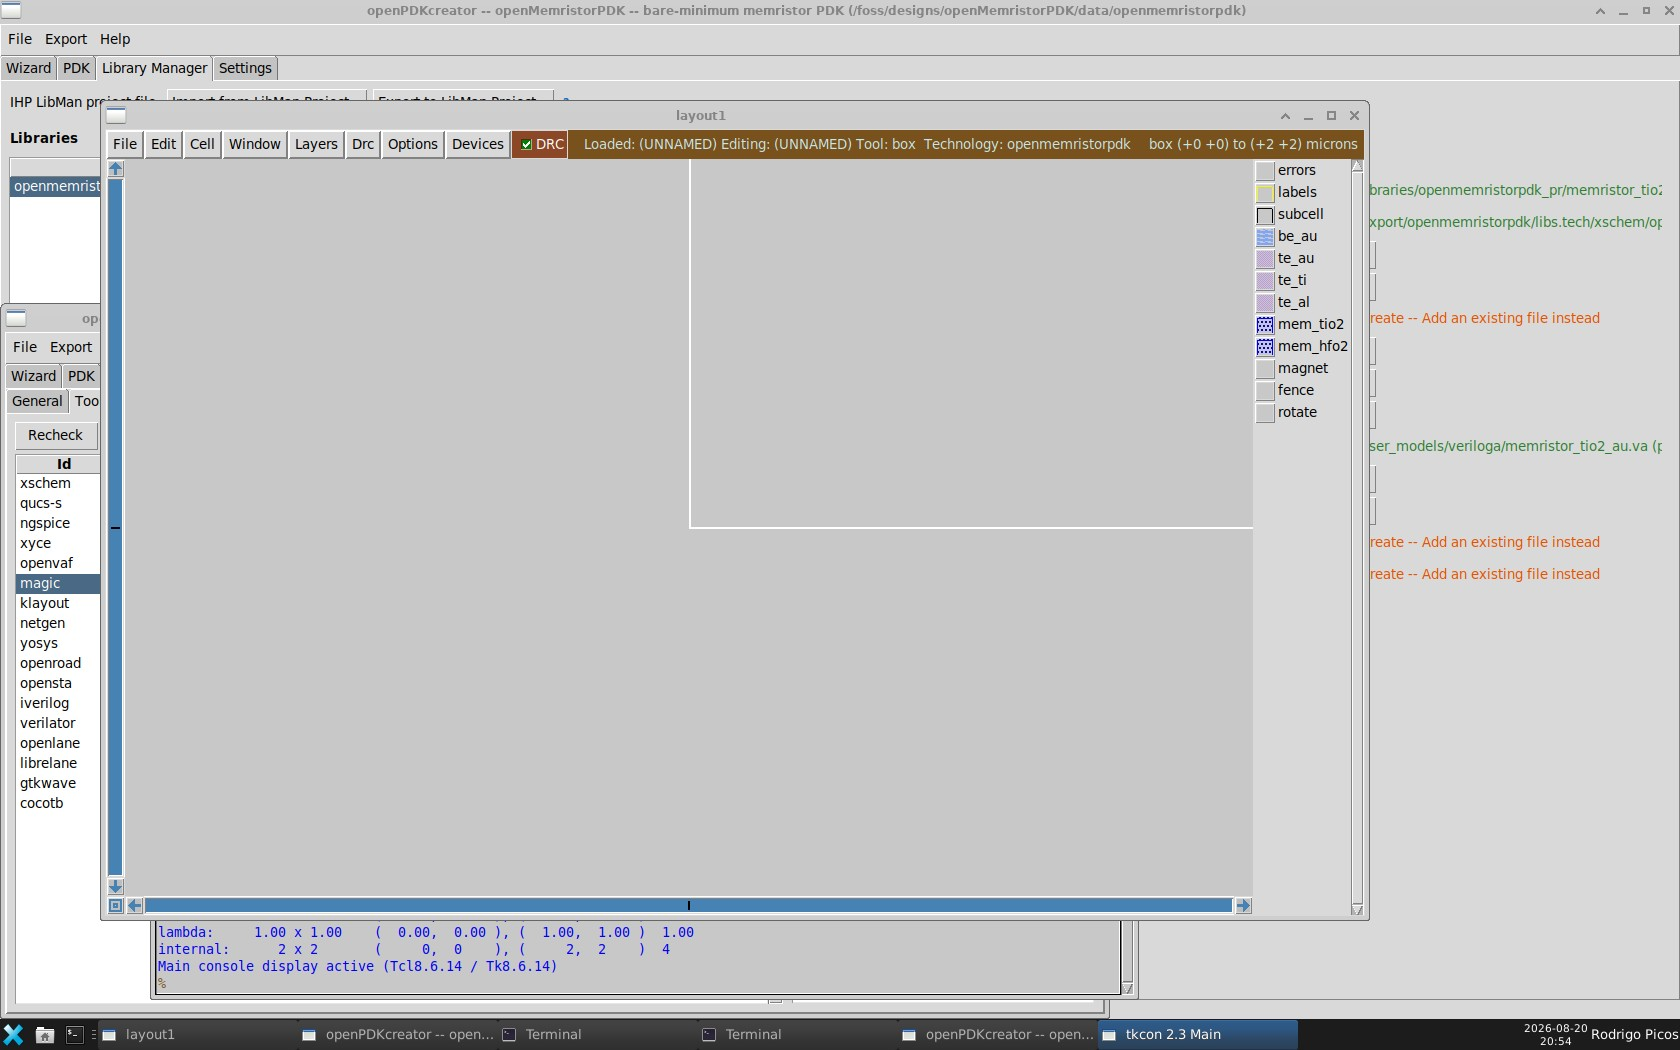
\includegraphics[width=0.7\textwidth]{figures/tooldeck_tools_view_magic.jpg}
\end{center}
\footnotesize
Not LibreLane itself (a real batch run takes too long for a single
illustrative screenshot) -- but the same real principle, shown for
Magic instead: this project's own \textbf{Settings $\to$ Tools $\to$
Launch Selected} button (a second, separate real launch path this
project found and fixed alongside the Library Manager's own buttons)
correctly shows \texttt{Technology: openmemristorpdk} too, confirming
both real launch paths -- and, by the same real logic, LibreLane's own
real \texttt{--pdk-root}/\texttt{--pdk} -- agree.
\end{frame}

% =================================================================
\section{Summary}
\begin{frame}[fragile]{Every real tool, every real flag, at a glance}
\footnotesize
\begin{center}
\begin{tabular}{lll}
\toprule
Tool & Real flag(s) this project passes & Real purpose \\
\midrule
Magic & \texttt{-d XR -rcfile <script>} & display driver; real, generated \texttt{tech load} \\
xschem & \texttt{--rcfile <rc> <file>} & real, correct \texttt{XSCHEM\_LIBRARY\_PATH} \\
KLayout (view) & \texttt{-l <lyp> -rr <script>} & real layer props; stay-open automation \\
KLayout (DRC) & \texttt{-b -r <script> -rd \dots} & real, structurally-safe batch mode \\
Qucs-S & \texttt{\$XDG\_CONFIG\_HOME=<tmp>} & real, disposable \texttt{QucsHomeDir} redirect \\
ngspice & \texttt{-b}, \texttt{pre\_osdi} & real batch sim; real OSDI load order \\
Netgen & \texttt{-batch source <script>} & real, device-level LVS \\
Yosys & \texttt{-c <script> -Q} & real synthesis script; safe by design \\
OpenROAD & \texttt{-exit -no\_splash -metrics} & real PnR/STA; \texttt{-no\_init} gap closed one level up \\
LibreLane & \texttt{--manual-pdk --pdk-root --pdk} & real, explicit, structurally safest of all \\
\bottomrule
\end{tabular}
\end{center}
\normalsize
Every one of these was checked against the real tool's own real
documentation or real source -- never guessed, and several real
mistakes (an empty \texttt{<tip-window-hidden/>} tag, a wrong return
type, a wrong argument order) were caught and fixed exactly this way,
not by assuming a first guess was right.
\end{frame}

\begin{frame}
\centering\Large Thanks!
\end{frame}

\end{document}
